\documentclass{article}

\input{0. Packages}
\newdateformat{monthyeardate}{%
  \monthname[\THEMONTH], \THEYEAR}


\title{Ice \& Climate \\ \vspace{1em} \large Assignment 1: Surface Energy Budget \normalsize}
\author{Yvo Werner\\ 9090649 } 
\date{October 2024}

\renewcommand{\arraystretch}{1.25}

\hfuzz=200pt



\begin{document}


\maketitle

\section{Research Question}
This report focuses on the investigation of the effects of changing ice/snow albedo values. 
More specifically, the prescription of albedo values $\alpha= 0.85, 0.7, 0.3$ are evaluated. 
In reality, changes in this parameter can represent a variety of processes. 
For one, it can represent varying degrees of snow coverage. 
This is the case because snow, ice and the ground below have different levels of albedo. 
Snow, especially freshly fallen snow, is highly reflective for the short wavelengths of the incoming solar radiation, so it has the highest albedo values of 0.8 to 0.9. 
As the snow ages its reflective properties become weaker and the albedo decreases. This is caused by impurities settling on the snow such as debris from surrounding open ground areas or advected dust. 
Also, events far away can have this effect: the large bushfires in Australia were shown to reduce albedo values on the glaciers of New Zealand due to the deposition of soot (\cite{Pu.2021}). 
Typical albedo values for this case are values of roughly 0.6 to 0.7. 
Another way of having a reduced surface albedo is by the emergence of glacier ice from underneath the snow layer. 
The process of compacting the snow and the recurring melting and freezing increases the albedo to values of 0.3 to 0.4.
Lastly, the presence of melt water on top of the ice would reduce the albedo even further. 
Liquid water has a much smaller albedo than its solid counterpart with albedo values ranging between 0.03 and 0.1 depending on the angle of solar radiation to the surface.\\
Thus, the research question of this project focuses on different areas of the research area, assuming different levels of snow and ice coverage, ranging from freshly fallen snow to exposed glacier ice. \\
The hypothesis of this report is that a lowering of the albedo will result in an increase of the surface temperature resulting in increased melt rates. 
To investigate this hypothesis, the Antartic Weather Station 14 was chosen due to its homogeneous surface and flat location with surface slopes of less than 0.1\textdegree (\cite{KuipersMunneke.2012}).
The research station is located on the Larsen C Ice Shelf at 67\textdegree00.8'~S 61\textdegree28.8' W sits about 55km from the ice shelf front to the east.


\section{Methodology}
This section provides the outline how changes in the albedo affect the components of the surface energy budget. 
It will also introduce the assumptions, simplifications and omissions made in the scope of this work and how they were implemented computationally.
The surface energy budget that is used here can be written as:
\begin{equation} \label{eq:SEB}
  M_{surf} = SW_{down} + SW_{up} + LW_{down} + LW_{up} + SHF + LHF + Gs
\end{equation}
where \vspace{-0.5\baselineskip}
\begin{itemize}[noitemsep]
  \item $M_{surf}$ is the surplus of energy available to melt the surface.
  \item $SW_{down}$ is the incoming shortwave radiation. 
  \item $SW_{up}$ is the outgoing shortwave radiation. 
  \item $LW_{down}$ is the incoming longwave radiation. 
  \item $LW_{up}$ is the outgoing longwave radiation.
  \item $SHF$ is the sensible heat flux. 
  \item $LHF$ is the latent heat flux. 
  \item $Gs$ is the ground heat flux.
\end{itemize}
The following subsections will now introduce the effects of changes in the albedo on each of these components and how they were implemented in the model.

\subsection*{Shortwave Radiation}

The only immediate impact of changes in the albedo are seen in the shortwave radiation budget. 
The albedo describes the amount of shortwave radiation that is reflected by the surface. 
If we now introduce a variable $SW_{net}$ that describes the energy flux that is retained at the surface, we can directly relate the incoming shortwave radiation to the retained radiation via the albedo parameter $\alpha$:
\begin{equation} \label{eq:SWNet}
  SW_{net} = \frac{SW_{up}}{SW_{down}} = SW_{down} * (1-\alpha)
\end{equation}
Changes to the albedo parameter thus have a direct impact on the amount of energy that is retained in the surface and the next subsections will focus on the changes these surplus or reduction of energy has on the other components in the SEB. \\
Computationally, these changes were implemented by using the measured downwelling shortwave radiation and applying three different values of albedo ($\alpha = 0.3, 0.7, 0.85$) in equation \eqref{eq:SWNet}. 

\subsection*{Longwave Radiation}

The two most dominant terms in equation \eqref{eq:SEB} are the net shortwave and net longwave radiation which is why --- to a rough leading order approximation --- a radiation balance is often applied between the incoming SW radiation and outgoing LW radiation. 
In other words, incoming SW radiation that is absorbed by the surface is largely balanced by the outgoing LW radiation. 
The energy flux of longwave radiation is described by the Stefan-Boltzmann relation:
\begin{equation*}
  LW_{up} = - \sigma T^4_{surface}
\end{equation*}
where \vspace{-0.5\baselineskip}
\begin{itemize}[noitemsep]
  \item $\sigma = 5.67 * 10^{-8}~W/m^2K^4$ is the Stefan-Boltzmann constant.
  \item $T_{surface}$ is the surface temperature in Kelvin.
\end{itemize}
This means that changes in the absorbed shortwave radiation cause changes in the temperature of the surface. \\
The incoming longwave radiation, however, is assumed to remain unchanged. 
This is due to the fact that the incoming longwave radiation is a function of the air temperature above the surface (usually paramterized as a function of the air temperature at 2m height). 
In reality, changes in the surface temperature will naturally also affect the 2m air temperature since the air is either heated or cooled from below. 
However, this process is further complicated by the presence of wind that is able to cool the surface by moving away already heated air, making an inclusion of this effect into the model more challenging. 
For the considerations of this project, we will thus treat $LW_{down}$ as an external forcing. \\
Computationally, changes in $LW_{up}$ were modelled using the linearised relationship given in the project description:
\begin{equation*}
  LW_{up}(T_{surf}^{adj}) = - \sigma {T_{surf}^{est}}^4- 4\sigma {T_{surf}^{est}}^3 (T_{surf}^{adj} - T_{surf}^{est}))
\end{equation*}
where \vspace{-0.5\baselineskip}

\begin{itemize}[noitemsep]
  \item $T_{surf}^{adj}$ is the adjusted surface temperature.
  \item $T_{surf}^{est}$ is the estimated surface temperature.
\end{itemize}

% In order to find the adjusted surface temperature the following equation was iteratively solved: 
% \begin{equation*}
%   M_{\text{surf}}^{\text{adj}} = SW_{\text{down}}^{\text{adj}} + SW_{\text{up}}^{\text{adj}} + LW_{\text{down}}^{\text{adj}} + LW_{\text{up}}(T_{\text{surf}}^{\text{adj}}) + SHF(T_{\text{surf}}^{\text{adj}}) + LHF(T_{\text{surf}}^{\text{adj}}) + G_s.
% \end{equation*}




\subsection*{Sensible Heat Flux}
The sensible heat flux represents heat transfer between the surface and the atmosphere due to temperature differences. 
In case that the surface is warmer than the air above it, heat is transferred from the surface to the air, effectively cooling the surface. 
Using the provided description, the sensible heat flux (SHF) is modelled by:
\begin{equation}\label{eq:SHF}
  SHF = c_s U_{10m} (T_{2m} - T_{surface})
\end{equation}
where \vspace{-0.5\baselineskip}
\begin{itemize}[noitemsep]
  \item $c_s$ is an exchange coefficient.
  \item $U_{10m}$ is the wind speed at 10m above the surface.
  \item $T_{2m}$ is the air temperature at 2m above the surface.
  \item $T_{surface}$ is the surface temperature.
\end{itemize}
It is thus apparent that changes in the surface temperature will also affect the sensible heat flux. 
Due to its linear dependence on the surface temperature (rather than a quadratic one in case of the LW radiation), the effects of a change can be expected to be much smaller. 
Nonetheless, its changes are still modelled using the linear relationship derived in the project description:
\begin{equation}\label{eq:SHF_linear}
  SHF(T_{surf}^{adj}) = SHF^{SEB} + c_s U_{10m} (T_{surf}^{SEB} - T_{surf}^{adj})
\end{equation}
where \vspace{-0.5\baselineskip}
\begin{itemize}[noitemsep]
  \item $SHF^{SEB}$ is model output of SHF under unaffected conditions.
  \item $T_{surf}^{SEB}$ is modelled surface temperature under unaffected conditions.
\end{itemize}
For this, first the exchange coefficient was determined with equation \eqref{eq:SHF}. 
Unfortunately, for AWS14 no direct measurements of the SHF were available so $c_s$ was calculated using the modelled SHF. 
With this, the SHF could then be adjusted iteratively by using equation \eqref{eq:SHF_linear}.


\subsection*{Latent Heat Flux}
The latent heat flux describes the heat transfer that takes place due to condensation of sublimation of water on the surface. 
The main gradient driving this process is the humidity gradient. 
Encapsulated in the Clausius-Clapeyron relation, surface temperature also influences this process, although to a smaller degree than in the case of the sensible heat flux.
In a similar formulation to the sensible heat flux, the latent heat flux is defined as: 
\begin{equation*}
  LHF = c_l U_{10m} (Q_{2m} - Q_{surface})
\end{equation*}
where \vspace{-0.5\baselineskip}
\begin{itemize}[noitemsep]
  \item $c_l$ is an exchange coefficient.
  \item $U_{10m}$ is the wind speed at 10m above the surface.
  \item $Q_{2m}$ is the specific humidity at 2m above the surface.
  \item $Q_{surface}$ is the specific humidity at the surface.
\end{itemize}
Since no observations of $Q_{surface}$ are available, the relative humidity and saturated specific humidity, a function of temperature and pressure, are used to calculate the LHF:
\begin{equation}\label{eq:LHF}
  LHF = c_l U_{10m} (RH_{2m}Q_{sat}(T_{2m}, P) - Q_{sat}(T_{surface}, P))
\end{equation}
\begin{itemize}[noitemsep]
  \item $c_l$ is an exchange coefficient.
  \item $U_{10m}$ is the wind speed at 10m above the surface.
  \item $Q_{sat}$ is the saturated specific humidity.
  \item $P$ is the measured air pressure.
\end{itemize}
Similar to the SHF, no measurements of the LHF were available for this weather station so the modelled values of LHF were used instead to calculate $c_l$ from equation \eqref{eq:LHF}.
Again, assuming $T_{2m}$ as constant, the adjusted LHF could then be calculated by plugging in the corresponding values into \eqref{eq:LHF}.

\subsection*{Omissions}
In accordance to the project description, any changes to the ground heat flux $Gs$ and shortwave radiation penetration have not been modelled in this case. 






% Unfortunately no observations of the SHF were provided for AWS14. 

% SHF_down_obs not found -> exhange coefficient was calculated using modelled SHF


\section*{Results}
In the following subsections the results of the surface energy budget are discussed. 
In the first subsection, the albedo for AWS14 is calculated in order to provide a context for the results found in the subsequent subsections. 
This is followed by the results for the melt, surface temperature and sensible heat flux. 


\subsection*{Albedo}
As previously mentioned, this subsection is concerned with the results of the albedo calculations for observed values of downward and upward shortwave radiation.
Using equation \eqref{eq:SWNet}, the albedo can easily be calculated from the observations. 
The result is shown in figure \ref{fig:Albedo} and they show that the albedo for AWS14 is generally in the range between 0.8 and 0.9 with few outliers up to 0.5. 
This means that the highest albedo scenario ($\alpha = 0.85$) roughly corresponds to the case present at AWS14. 
The sensitivity analysis is concerned with the effects of a slight drop in the albedo compared to original values ($\alpha = 0.7$), e.g. through the presence of dust or soot on the ice and the effects of a sharp drop in the albedo ($\alpha = 0.3$) which could, for example, correspond to the case where melt water is present on the surface of the ice.

\begin{figure}[h!]
  \centering
  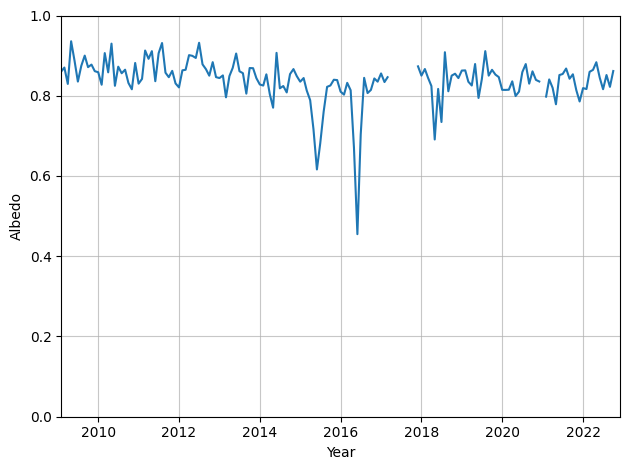
\includegraphics[width=0.8\textwidth]{figures/Albedo.png}
  \caption{Albedo values (blue line) calculated from observations of incoming and outgoing shortwave radiation using equation \eqref{eq:SWNet}.}
  \label{fig:Albedo}
\end{figure}

\subsection*{Accumulated Melt}
This subsection is concerned with the effects of changes in the albedo on the accumulated melt (see Figure \ref{fig:AccMelt}).
As previously discussed, results for $\alpha = 0.85$ are expected to resemble the original model results, which can be confirmed.
The black line (the original model result) and the green line in Figure \ref{fig:AccMelt} (the model result for $\alpha = 0.85$) follow each other closely. 
However, there is a deviation happening in the time span between 2015 and 2016. 
This can be explained with the outliers present in the observed albedo (see Figure \ref{fig:Albedo}) happening at the same time. 
These outliers cause the observed melt to increase drastically explaining the seperation. 
Since observed albedo values return to normal shortly after, the lines do not seperate further but remain rather parallel thereafter. \\
For the slight decrease in albedo ($\alpha = 0.7$), an overall increase in melt can be seen (orange line in Figure \ref{fig:AccMelt}). 
This is to be expected as more shortwave radiation is retained in the surface, increasing the surface temperature and providing ultimately more energy that is availble for the melting process. \\ 
The most notable difference can be seen for $\alpha = 0.3$ (blue line in Figure \ref{fig:AccMelt}). 
Here, melt increases more than tenfold, really showcasing the strong influence of the albedo on the presence of melting. 
Additionally, the melt profile shows the characteristics plateaus that are to be expected due to seasonal differences of incoming shortwave radiation. 
The absence of virtually any shortwave radiation input during the polar night, results not only in a diminishing influence of the albedo during this time but also in the absence of melting. 
In other words, little or none melting takes place during the polar night which causes all lines to be parallel during the Antarctic winter (visualised by the plateaus) but the melting process is much more pronounced during the Antarctic summer when the sun shines all day (visualised by the strong increases).

\begin{figure}[h!]
  \centering
  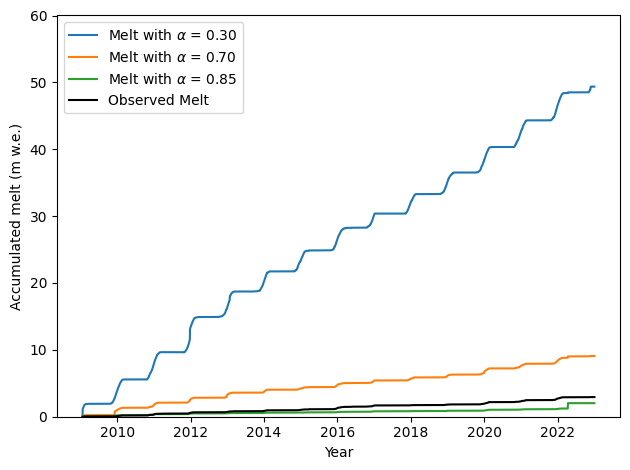
\includegraphics[width=0.8\textwidth]{figures/MeltCum.png}
  \caption{Accumulated melt for the three different albedo values $\alpha = 0.85, 0.7, 0.3$. The black line corresponds to the original model results without prescribing a fixed albedo value.}
  \label{fig:AccMelt}
\end{figure}

\subsection*{Surface Temperature}
This section is concerned with the effects of changing albedo values on the modelled surface temperature. 
As previously mentioned, the surface temperature is directly influenced by changes in the retained shortwave radiation due to the fact that the surface balances the incoming shortwave radiation by emitting longwave radiation. 
Thus, a surplus in shortwave radiation is compensated by a increase in surface temeprature and vice versa. 
Considering this, it can be expected that the surface temperature will increase as more shortwave radiation is retained in the surface when succesively lowering the albedo. \\
\begin{figure}[h!]
  \centering
  % Top subfigures
  \begin{subfigure}{0.49\textwidth}
      \centering
      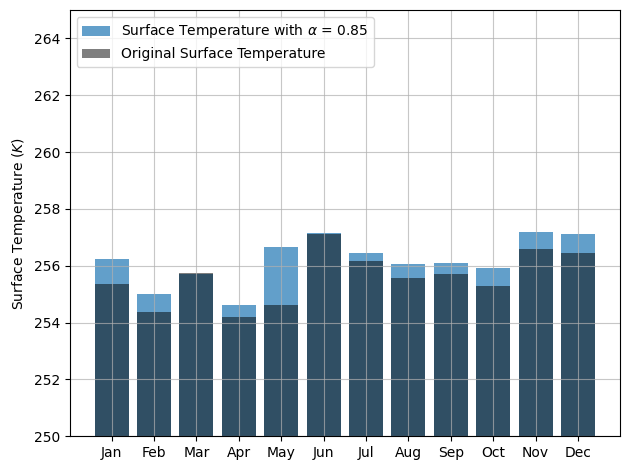
\includegraphics[width=\linewidth]{figures/Bar_Tsurf_085.png}  % Replace with your image
      \caption{Surface Temperatures for $\alpha = 0.85$}
      \label{fig:SurfaceTemp085}
  \end{subfigure}
  \hfill
  \begin{subfigure}{0.49\textwidth}
      \centering
      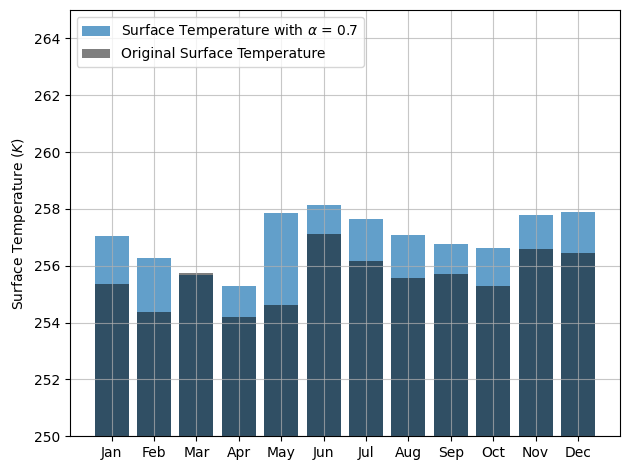
\includegraphics[width=\linewidth]{figures/Bar_Tsurf_07.png}  % Replace with your image
      \caption{Surface Temperatures for $\alpha = 0.7$}
      \label{fig:SurfaceTemp07}
  \end{subfigure}
  
  % Below subfigure
  \vspace{1cm}  % Adjust the space between the two rows
  \begin{subfigure}{0.5\textwidth}
      \centering
      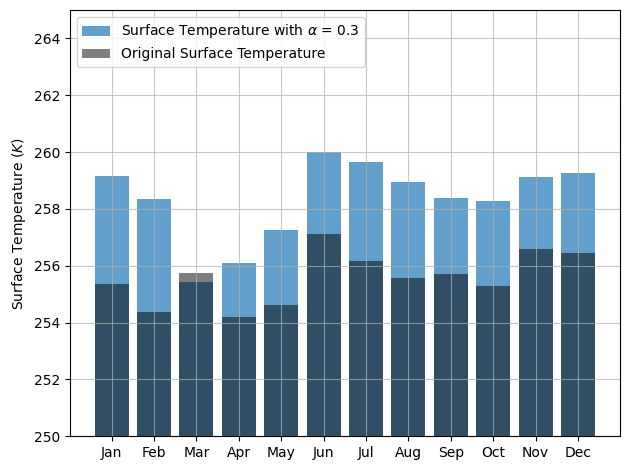
\includegraphics[width=\linewidth]{figures/Bar_Tsurf_03.png}  % Replace with your image
      \caption{Surface Temperatures for $\alpha = 0.3$}
      \label{fig:SurfaceTemp03}
  \end{subfigure}
  
  \caption{Monthly surface temperatures for the three different albedo scenarios ($\alpha = 0.85, 0.7, 0.3$). The monthly averages were computed from data available between 21-01-2009 and 01-01-2023.}
  \label{fig:SurfaceTemp}
\end{figure}
This assumption is verified by the sensitivity results shown in Figure \ref{fig:SurfaceTemp}. 
More specifically, Figure \ref{fig:SurfaceTemp085} shows that when the albedo is set close to the observed one ($\alpha = 0.85$), surface temperatures deviate only slightly. 
As expected, the strong deviations can be found during summer and spring when the sun shines most and any differences between the prescribed albedo and the actual one are most pronounced. 
For the slightly reduced case, $\alpha = 0.7$, an overall increase in surface temperatures can be seen (see Figure \ref{fig:SurfaceTemp07}). 
As previously discussed, this is due to the increased shortwave radiation retained by the surface. 
The strongest increases in surface temperature are visible for the lowest albedo value (see Figure \ref{fig:SurfaceTemp03}).
Here, surface temperatures (with the exception of March) are generally at least two degrees warmer when compared to the reference case. 
This helps explain the large values of melt that were seen in the previous section. 
The March outlier is most likely due to a computational error where the exchange coefficient of sensible heat flux and latent heat flux became extremely large. 
This reduced the overall number of available data points drastically and could explain the relative absence of any behaviour in all three scenarios. 



\subsection*{Sensible Heat Flux}
This section is concerned with the effects of the changing albedo on the sensible (and latent) heat flux. 
Although overall much less important than the longwave radiation response, it is still included because it can help explain why we see increased surface temperatures even during the polar night when the albedo effects shouldn't be visible anymore. 

\begin{figure}[h!]
  \centering
  % Top subfigures
  \begin{subfigure}{0.49\textwidth}
      \centering
      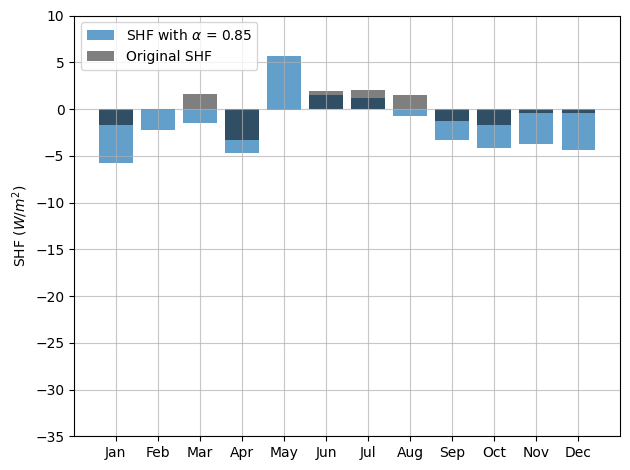
\includegraphics[width=\linewidth]{figures/Bar_SHF_085.png}  % Replace with your image
      \caption{SHF for $\alpha = 0.85$}
      \label{fig:SHF085}
  \end{subfigure}
  \hfill
  \begin{subfigure}{0.49\textwidth}
      \centering
      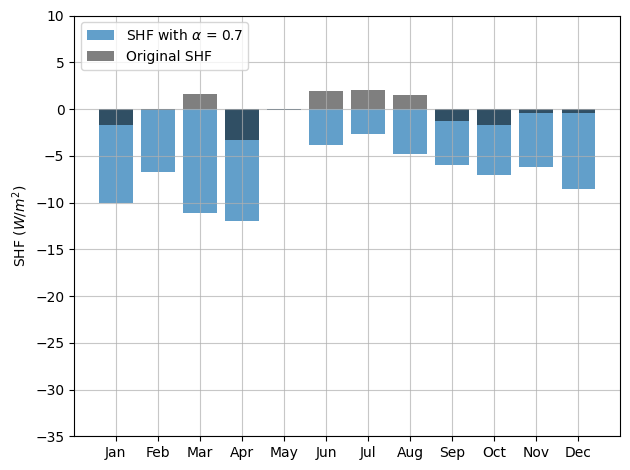
\includegraphics[width=\linewidth]{figures/Bar_SHF_07.png}  % Replace with your image
      \caption{SHF for $\alpha = 0.7$}
      \label{fig:SHF07}
  \end{subfigure}
  
  % Below subfigure
  \vspace{1cm}  % Adjust the space between the two rows
  \begin{subfigure}{0.5\textwidth}
      \centering
      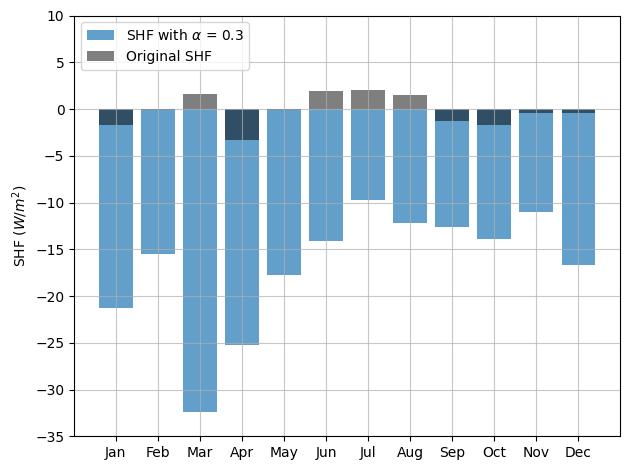
\includegraphics[width=\linewidth]{figures/Bar_SHF_03.png}  % Replace with your image
      \caption{SHF for $\alpha = 0.3$}
      \label{fig:SHF03}
  \end{subfigure}
  
  \caption{Monthly averages for the sensible heat flux (SHF) in dependence on the three different albedo values ($\alpha = 0.85, 0.7, 0.3$). The monthly averages were computed from data available between 21-01-2009 and 01-01-2023.}
  \label{fig:SHF}
\end{figure}

While not explicitly shown here, the same considerations below also hold true for the latent heat flux. 
Because the latent heat flux is generally smaller than the sensible heat flux, the latter will be the object of discussion for this section. 
In a similar plot to that of the surface temperature, the results can be seen in Figure \ref{fig:SHF}. 
Overall, we can see an increase in the magnitude of the SHF as the albedo decreases. 
Considering the negative sign, this implies that the SHF is directed away from the surface. 
Applied to the scenario at hand, this means that as the albedo decreases, the SHF provides an increasing pathway for the surplus of energy from the surface to the atmosphere above. 
This behaviour is partly caused by the assumptions made for this sensitivity analysis. 
In the methodology section, we assumed that the air temperature above the surface remains unaffected by any increases to the surface temperature. 
Since the difference between both temperatures is the driving factor in the magnitude of the SHF this means that it increases drastically as the 2m air temperature is kept unchanged. 
Similar effects are seen for the latent heat flux due to its dependence on the saturation specific humidity which in turn is modulated by the air / surface temperature as well. 



\section*{Discussion}

The goal of this project was to investigate the effects of varying albedo values on the surface energy budget at AWS14 located on the Larsen C Ice Shelf in Antarctica.
More specifically, albedo values of 0.85, 0.7 and 0.3 were applied to demonstrate the important role that the albedo plays in determining surface energy fluxes and temperature. 
Overall, the connection between albedo and surface conditions is simple.
As albedo values decrease, more shortwave radiation is absorbed by the surface leading to a considerable increase in surface temperatures. 
This relationship ultimately connects the changes in albedo to differences in accumulated melt, surface temperatures and sensible and latent heat fluxes. \\
First, the context for evaluating the albedo was set by determining the albedo values present at AWS14 from observations. 
It was found that at this location, albedo values generally are between 0.8 and 0.9, meaning that the high albedo scenario evaluated in this case roughly corresponds to a long-term mean albedo at this location. \\
Next, the melt rates were evaluated where the most direct impact of lowering the albedo was apparent. 
Lowering the albedo to 0.3 resulted in enhanced melting, especially during the summer months when more energy was retained by the surface due to the reduced reflection of solar radiation. 
Overall, the surface energy budget shifted towards a net positive balance where the excess energy resulted in the enhanced melting. 
Conversely, an albedo value of 0.85 remained close to the melt values of the untouched case. 
The results for 0.7 represented an intermediate case where melting was significantly enhanced when compared to the high albedo case but not nearly as high as the low albedo case.\\
In the case of the sensible heat flux, lower albedo values lead to strongly negative values indicating an increased flux from the surface to the atmosphere. 
This is caused by the increase in surface temperatures leading to stronger temperature differences between air and surface, especially since the air temperatures were assumed to remain constant. 
At higher albedo values, the sensible heat flux remained relatively unaffected and compartively small indicating that surface and air were in much more thermal equilibrium and less heat was transferred from the surface to the air.\\
Overall, the findings of this project show the high sensitivity of the Antarctic surface energy budget to changes in the albedo where even slight reductions of the albedo can lead to disproportionate increases in surface temperature and snow melt. 
This is particularly important in the context of climate change as this can lead to positive feedback loops. 
One example of this is the presence of melt water on top of the ice sheet. 
Liquid water has a much lower albedo than snow or ice and thus causes the surface to absorb much more solar radiation. 
As shown in this project, this causes enhanced melt rates which in turn causes more melt water to be present at the surface. \\
Additionally, the results of this project highlight the importance of accurately calculating or prescribing the albedo in climate models and surface energy budget models. 
As previous results have shown, even slight deviations can cause non-linear ramifications in other parameters down the line; especially when more dependencies are taken into account.\\



\printbibliography



\section*{Appendix}

\lstinputlisting[caption = {Python code, Data Analysis}, basicstyle = \tiny]{appendix/SEB_Code.py}

\end{document}
